\subsection{Quantitative engagement audit: DrugCentral (third orthogonal null)}
DGIdb records interaction claims and Open Targets predicts tractability
buckets; DrugCentral (snapshot 2021\_09\_01,
\texttt{results/drugcentral\_engagement.json}) instead holds curated
\emph{quantitative} drug--target activities (ChEMBL-derived potencies and
FDA-label mechanisms) over 19,378 activity records, 14,301 of them human,
covering 1,704 human genes and 2,339 drugs. Applied to the same
99-gene gated set and 98-gene random-surfaceome background as the Open
Targets audit, the gate enriches for nothing: 17/99 gated antigens carry
any human activity record versus 19/98 background (odds 0.862, $p=0.72$);
6/99 versus 7/98 are Tclin (target of an approved-drug mechanism;
odds 0.839, $p=0.78$); 6/99 versus 8/98 carry a curated MOA record
($p=0.59$). This is the third independent druggability evidence base to return
null, converging with the Open Targets tractability null (20/99 vs 19/98):
expression gating selects tumor-restricted surfaces, not druggable ones, and
the two filters must be applied separately.

Controls behave as the snapshot dictates: CD19 returns four approved
biologics (blinatumomab, inebilizumab, loncastuximab tesirine, tafasitamab), all Tclin; ERBB2 is Tclin with 36 drugs. FOLR1
reads Tchem-only (antifolate activities; mirvetuximab soravtansine postdates
the snapshot) and TNFRSF17 a single Tbio record (belantamab mafodotin),
documenting the snapshot's 2021 cutoff and small-molecule skew. The AND-gate
antigens split sharply: CA9 and CA12 are heavily but \emph{promiscuously}
engaged (45 and 45 drugs respectively, headed by the carbonic-anhydrase
inhibitors acetazolamide and brinzolamide --- non-selective engagement that
argues for antigen gating rather than drugging of these targets), while
CLDN18, MSLN, CLDN6, PSCA, SLC39A6 return zero curated records, extending the DGIdb CLDN6
zero-engagement finding to five of the seven AND-gate candidates. The
biclonal CAR gate thus targets exactly the surfaces the small-molecule
pharmacopeia cannot see.

\begin{figure}[h]\centering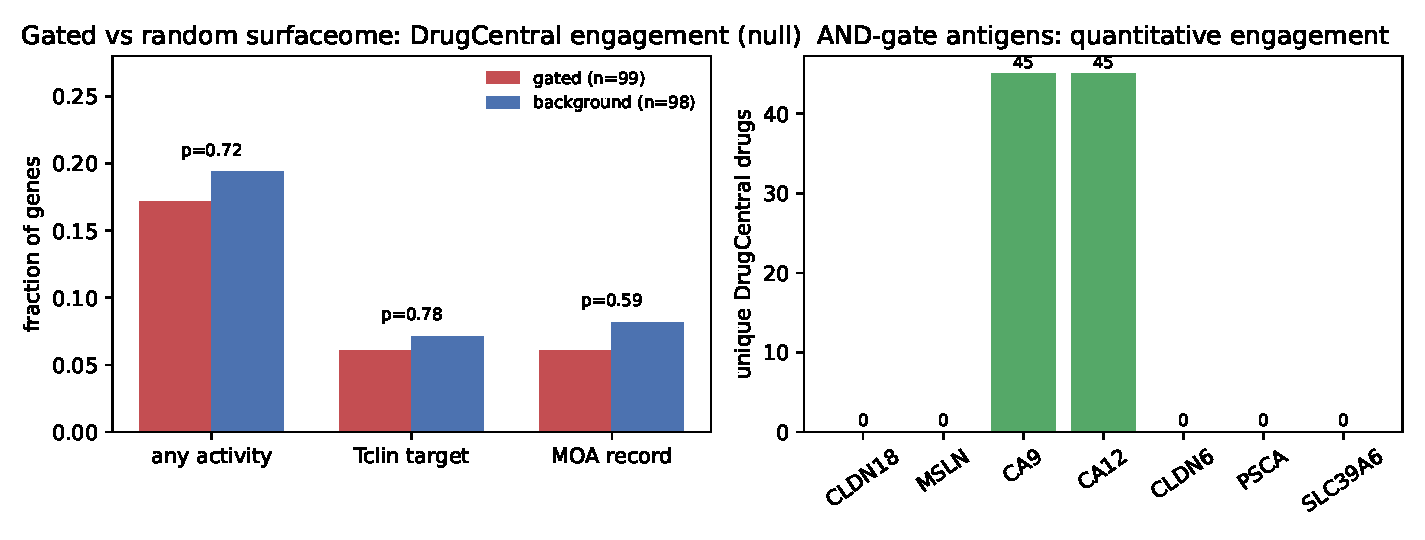
\includegraphics[width=0.98\linewidth]{figs/fig_drugcentral.pdf}
\caption{DrugCentral engagement audit. Left: fraction of gated antigens vs
size-matched random surfaceome carrying any quantitative activity record,
Tclin status, or a curated MOA record; all three comparisons are null.
Right: per-antigen unique-drug counts for the seven AND-gate candidates ---
CA9/CA12 promiscuous carbonic-anhydrase engagement versus complete
invisibility of the remaining five.}\end{figure}
